\documentclass[10pt,journal,compsoc]{IEEEtran}

\usepackage[pdftex]{graphicx}    
\usepackage{cite}
\hyphenation{op-tical net-works semi-conduc-tor}

\usepackage{listings}

\begin{document}

\title{Map My World Robot using RTAB-MAP}

\author{Peng Xu}

\markboth{SLAM project, Robotic Nanodegree, Udacity}%
{}
\IEEEtitleabstractindextext{%

\begin{abstract}
This project attempts to apply Simultaneous Localization and Mapping (SLAM) algorithms
in ROS and Gazebo, and discusses how and why the SLAM algorithms succeed or fail to solve
the problem. The SLAM algorithm used is Real Time Appearance Based Mapping (RTABMap), a type of GraphSLAM algorithm that uses traditional computer vision techniques to solve the correspondence problem. The algorithm works well in the first environment, where the map features are distinguishable from each other. However the mapping and localization accuracies were lower when the robot explores an environment with visually similar regions and failed to correlate different frames correctly.

\end{abstract}

% Note that keywords are not normally used for peerreview papers.
\begin{IEEEkeywords}
Robot, SLAM, RTAB-MAP, 3D Reconstruction, Loop Closure.
\end{IEEEkeywords}}


\maketitle
\IEEEdisplaynontitleabstractindextext
\IEEEpeerreviewmaketitle
\section{Introduction}
\label{sec:introduction}

\IEEEPARstart{I}{n} the real world, there are few scenarios where we can provide the robots with fully featured maps to navigate through the environments. The robots would need to localize themselves and map the environments at the same time. The technology to solve this problem is named Simultaneous Localization and Mapping (SLAM). This project continues the previous project on localization, and explores how the Simultaneous Localization and Mapping (SLAM) methods works in a simulated environment. The robot would be using a RGB-D camera and estimates its trajectory and map feature poses as it moves through the environment. If the SLAM algorithm is successful, the robot would be able to produce a map with identifiable features in the surroundings and its trajectory.

The project aims to create a 2D occupancy grid and 3D octomap from a provided simulated environment. Also, to further validate the method, a customized simulated environment would be created to be mapped as well.

\section{Background}

In navigation, robotic mapping and odometry, simultaneous localization and mapping (SLAM) is the computational problem of constructing or updating a map of an unknown environment while simultaneously keeping track of an agent's location within it. While this initially appears to be a chicken-and-egg problem there are several algorithms known for solving it, at least approximately, in tractable time for certain environments. Popular approximate solution methods include the particle filter, extended Kalman filter, Covariance intersection, and GraphSLAM.

A complete SLAM system performs a number of operations repeatedly. First, a set of new landmarks are detected in the environment, initialized (also referred as new landmark initialization), and inserted into the map. As the robot (i.e. observer) moves to a new location, observations are made and matched with the map landmarks, and this process is referred as data association. In case of a tracking failure, relocalization methods are used for recovery. Then, a prior estimation of the robot motion is obtained, this operation is referred as motion estimation. Next, the estimates of landmark positions and robot pose that best explains the data are isolated, eliminating the inaccurate estimates, this operation is referred as optimization. If a previously mapped portion of the environment is re-observed, the loop closure algorithm is executed. The sequence of operations that creates a SLAM system is as follows.

\begin{lstlisting}
Repeat
    1. Observation
    2. Data association
    if tracking failure is detected then
        3. Relocalization
    4. Motion estimation
    5. Optimization
    if loop closure is detected then
        6. Loop closure correction
\end{lstlisting}

\subsection{Laser-Based SLAM}

The laser rangefinder emits short pulses of infra-red laser light and measures how long it takes for the reflected pulse to return. The time-of-flight is used to calculate the distance. If the pose of the mobile robot is sufficiently well known through the onboard IMU or alternatively using the wheel encoders, then the laser scans can be transformed into global coordinate frame, which then can be used to build a map by employing a probabilistic approach. For a robot at a given pose, each range measurement in the scan determines the coordinates of a cell that contains an obstacle however the robot has no information about the cells that are behind the detected obstacles, these cells are registered as unknown cells whereas the cells that are between the sensor and the detected obstacles are registered as obstacle-free cells.

\subsection{Vision-Based SLAM}

Visual SLAM can be defined as the problem of building maps and tracking the robot pose in full 6-DOF using data from cameras (i.e. RGB-D sensors). RGB-D sensors offer the visual information that enables the construction of rich 3-D models of the world. They also enable difficult issues such as loop-closing to be addressed in novel ways using appearance information.

RTAB-Map (Real-Time Appearance-Based Mapping) is a RGB-D graph-based SLAM approach based on an incremental appearance-based loop closure detector. RTAB-Map represents the-state-of-art solution for SLAM to develop robots that can map environments in 3D. These considerations come from RTAB-Map's speed and memory management, its custom developed tools for information analysis and, most importantly, the quality of the documentation. For this project the rtabmap\_ros package will be used, which is a ROS wrapper (API) for interacting with rtabmap. Fig. \ref{fig:rtab-flow} illustrates the flowchart of the proposed method.

\begin{figure}[thpb]
      \centering
      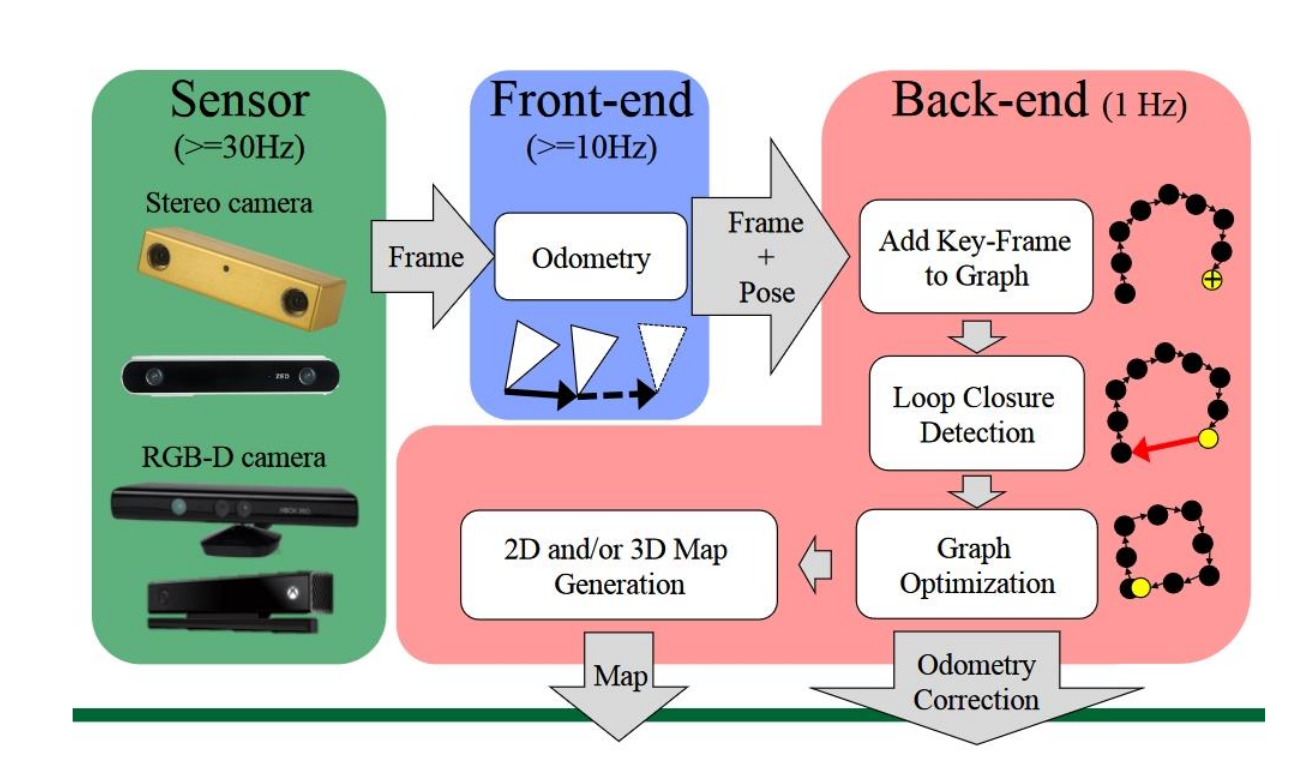
\includegraphics[width=\linewidth]{images/rtab-flow.png}
      \caption{Stages of the Real-Time Appearance-based Mapping (RTAB-Map)}
      \label{fig:rtab-flow}
\end{figure}

\section{Scene and robot configuration}

\subsection{Scene configuration}

A provided kitchen world is provided as in Fig. \ref{fig:kitchen-gazebo}

\begin{figure}[thpb]
      \centering
      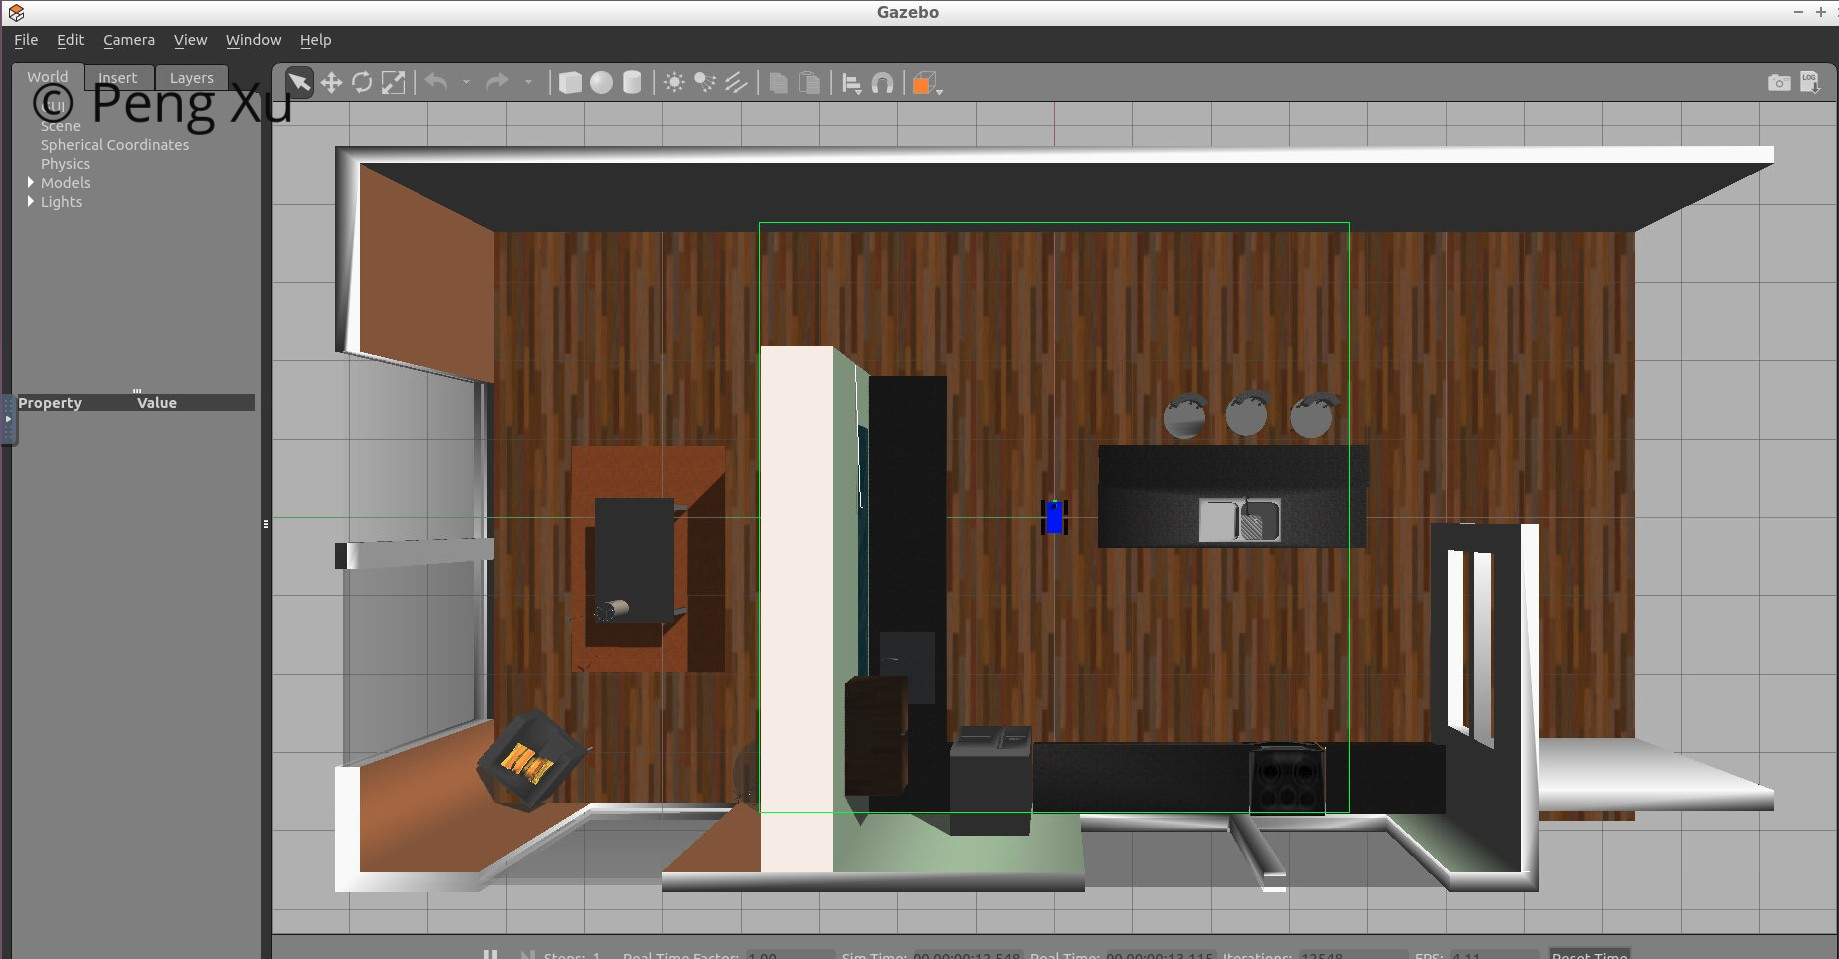
\includegraphics[width=\linewidth]{images/kitchen-gazebo.png}
      \caption{Kitchen World}
      \label{fig:kitchen-gazebo}
\end{figure}

A customized cafe world is built from scratch in Gazebo as in Fig. \ref{fig:cafe-gazebo}. The models in the scene are all from the online model database. To ensure the vision features distinguishable some other models such as tables are placed carefully in the cafe. In the meantime, enough room are remained for the robot to explore.

\begin{figure}[thpb]
      \centering
      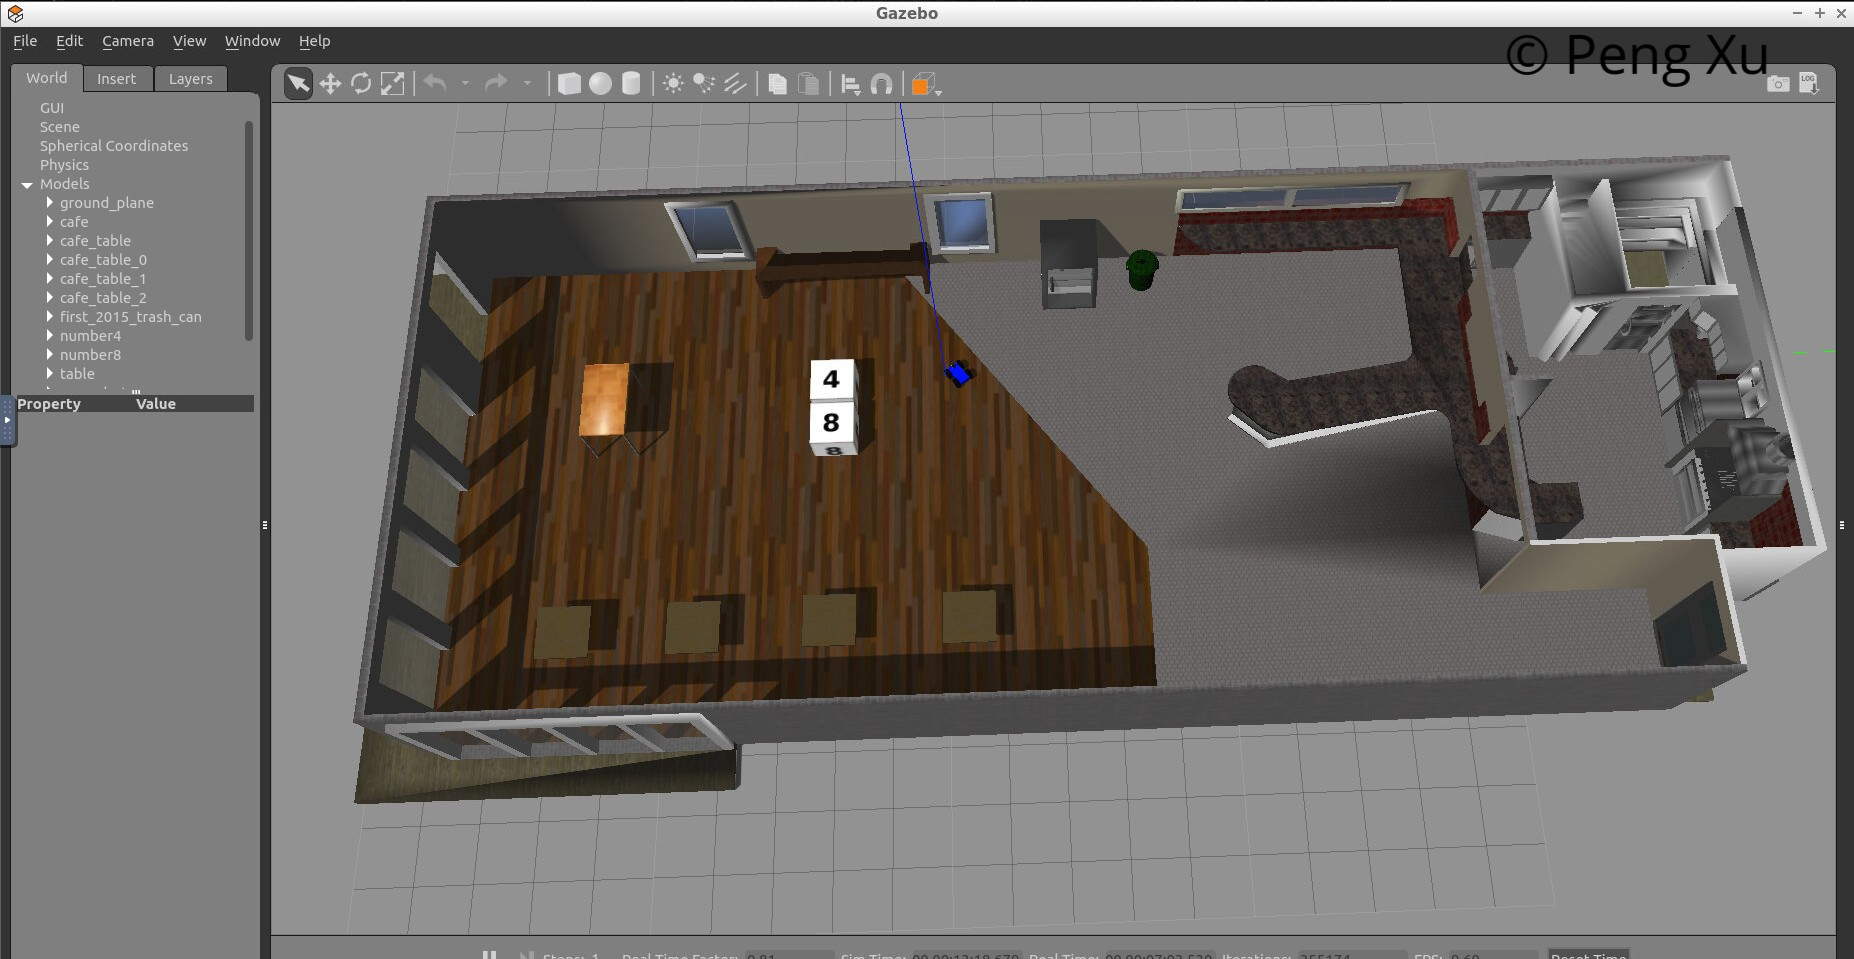
\includegraphics[width=\linewidth]{images/cafe-gazebo.png}
      \caption{Cafe World}
      \label{fig:cafe-gazebo}
\end{figure}

\subsection{Robot configuration}

The robot was inherited from the model in the previous project. The camera was required to be replaced by a RGB-D camera. From the point of view of the frame links as shown in Fig. \ref{fig:bot-frames}, a new RGB-D camera node in the .gazebo file was attached to the camera node.

\begin{figure}[thpb]
      \centering
      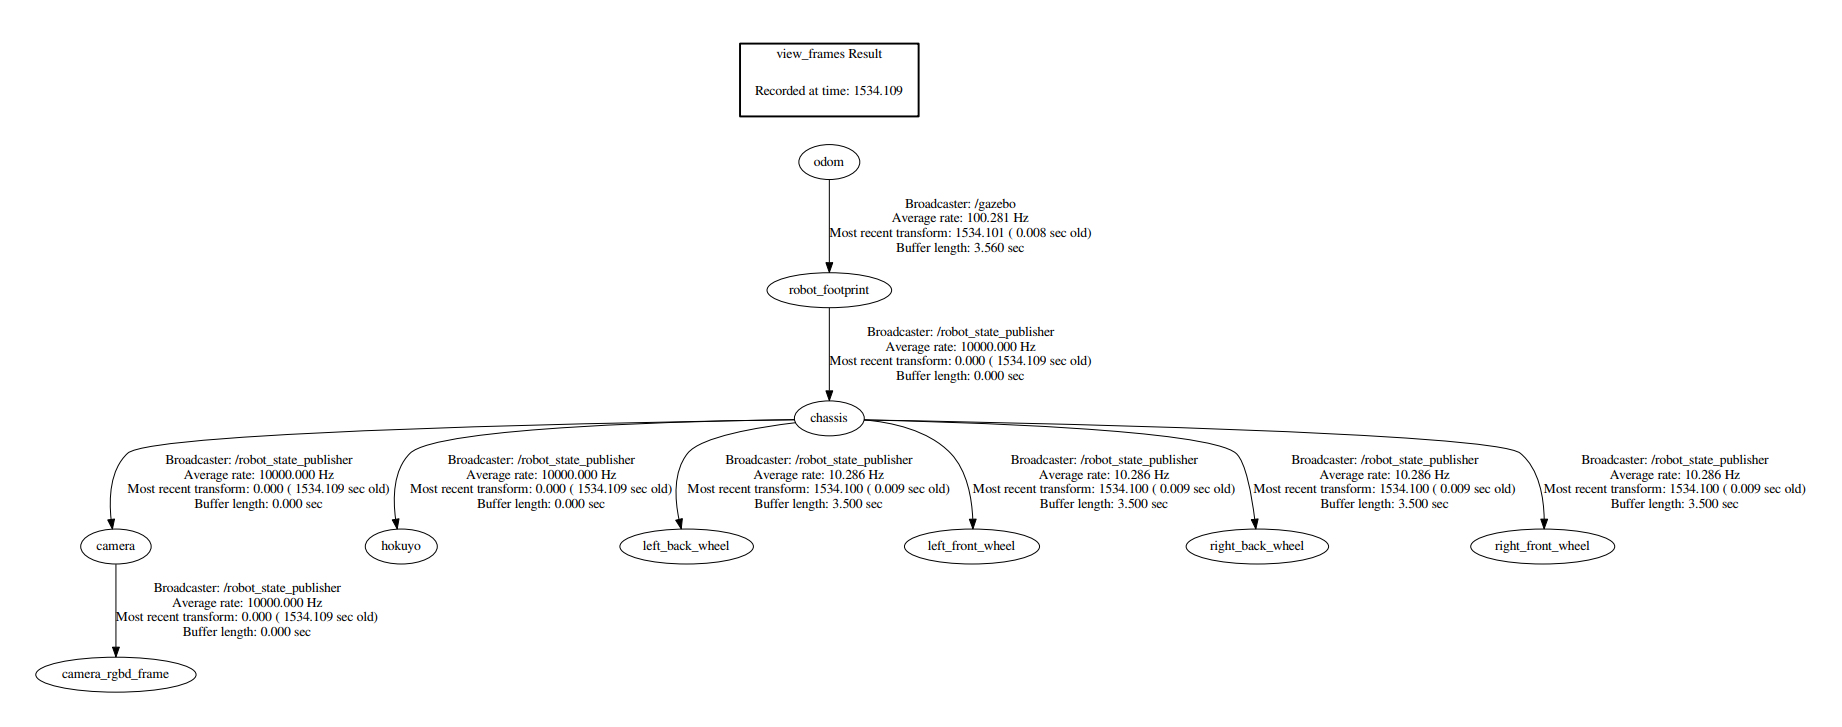
\includegraphics[width=\linewidth]{images/frames.png}
      \caption{Robot Frames}
      \label{fig:bot-frames}
\end{figure}

The following tree diagram depicts the package structure and files that made it up.

\begin{lstlisting}
.
├── CMakeLists.txt
├── launch
│   ├── localization.launch
│   ├── mapping.launch
│   ├── rviz.launch
│   ├── teleop.launch
│   └── world.launch
├── package.xml
├── rviz
│   └── robot_slam.rviz
├── script
│   ├── rtab_run
│   └── teleop
└── worlds
    ├── cafe_dining.world
    └── kitchen_dining.world
\end{lstlisting}

\section{Results}

\subsection{Kitchen World}

\begin{figure}[thpb]
      \centering
      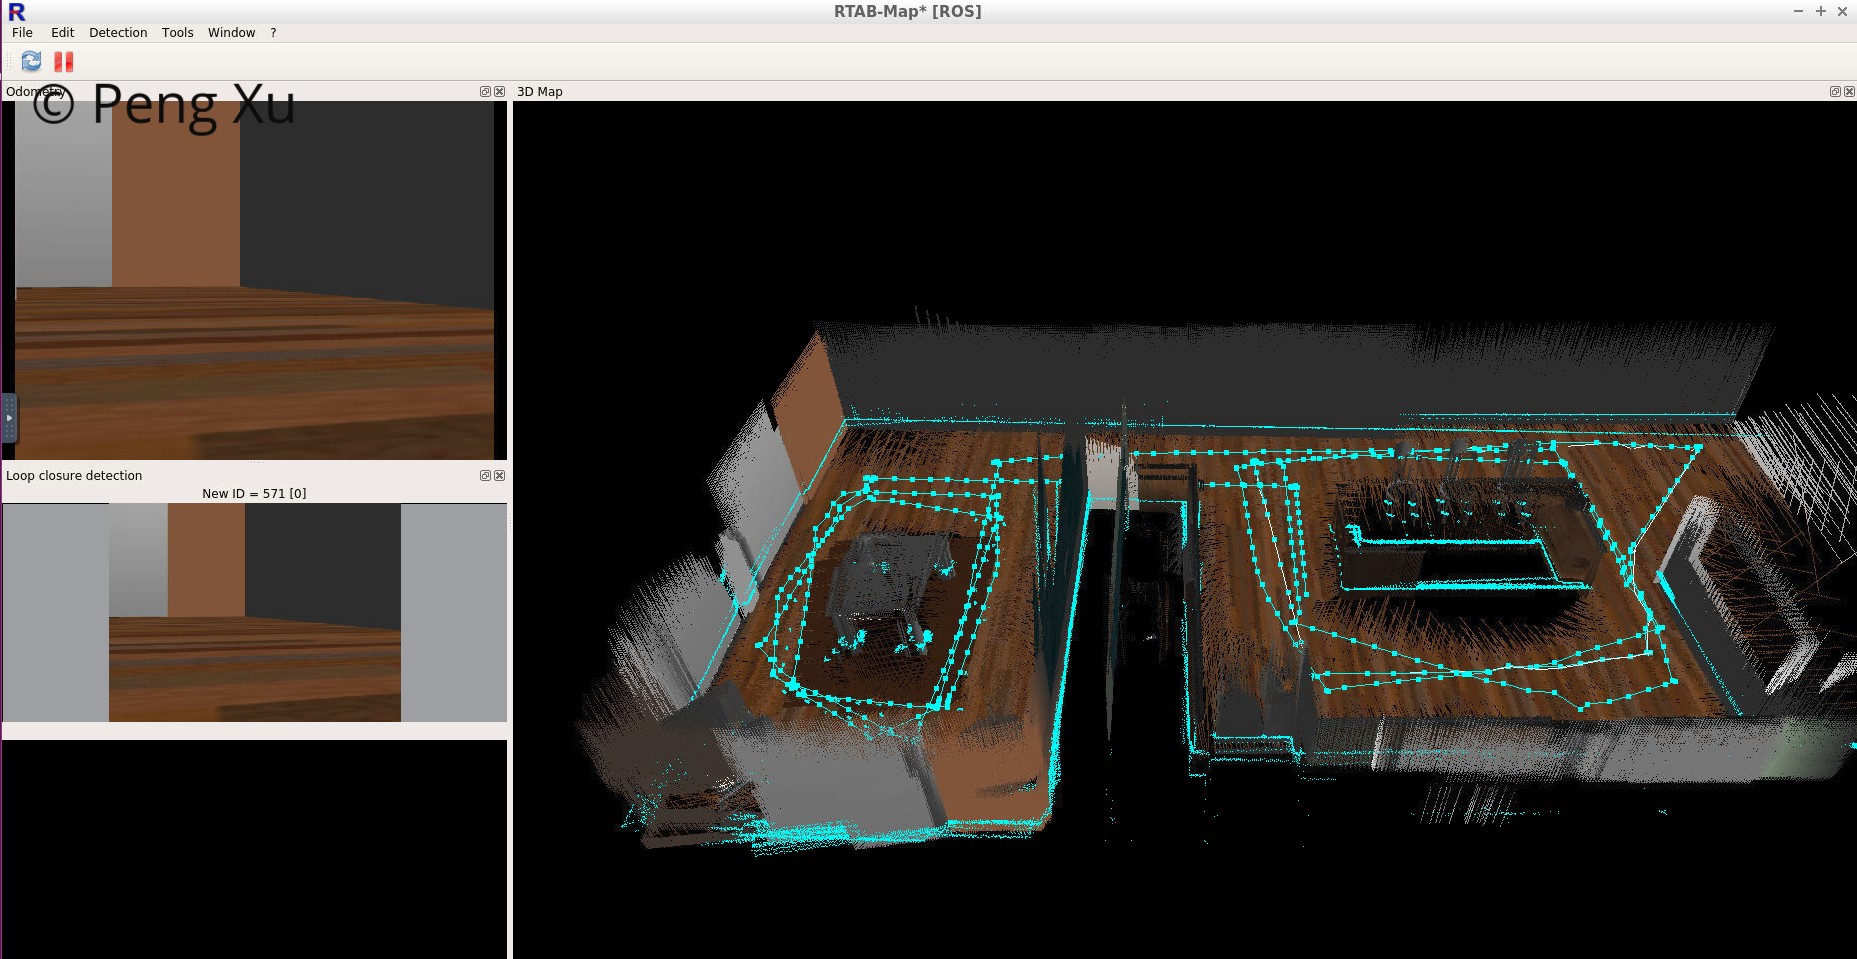
\includegraphics[width=\linewidth]{images/kitchen-rtab-map.png}
      \caption{RTAB Map of Kitchen World}
      \label{fig:kitchen-rtab-map}
\end{figure}

The 2D maps of both environments elicits the movable areas for the robot in the environment well as shown in Fig. \ref{fig:kitchen-rviz} and Fig. \ref{fig:cafe-rviz}. However, the 2D maps are produced from the scans of the laser rangefinder, which is mounted higher on the robot. As a result, it will only consider obstacles at the height of the laser rangefinder and omits some of the small objects.

\begin{figure}[thpb]
      \centering
      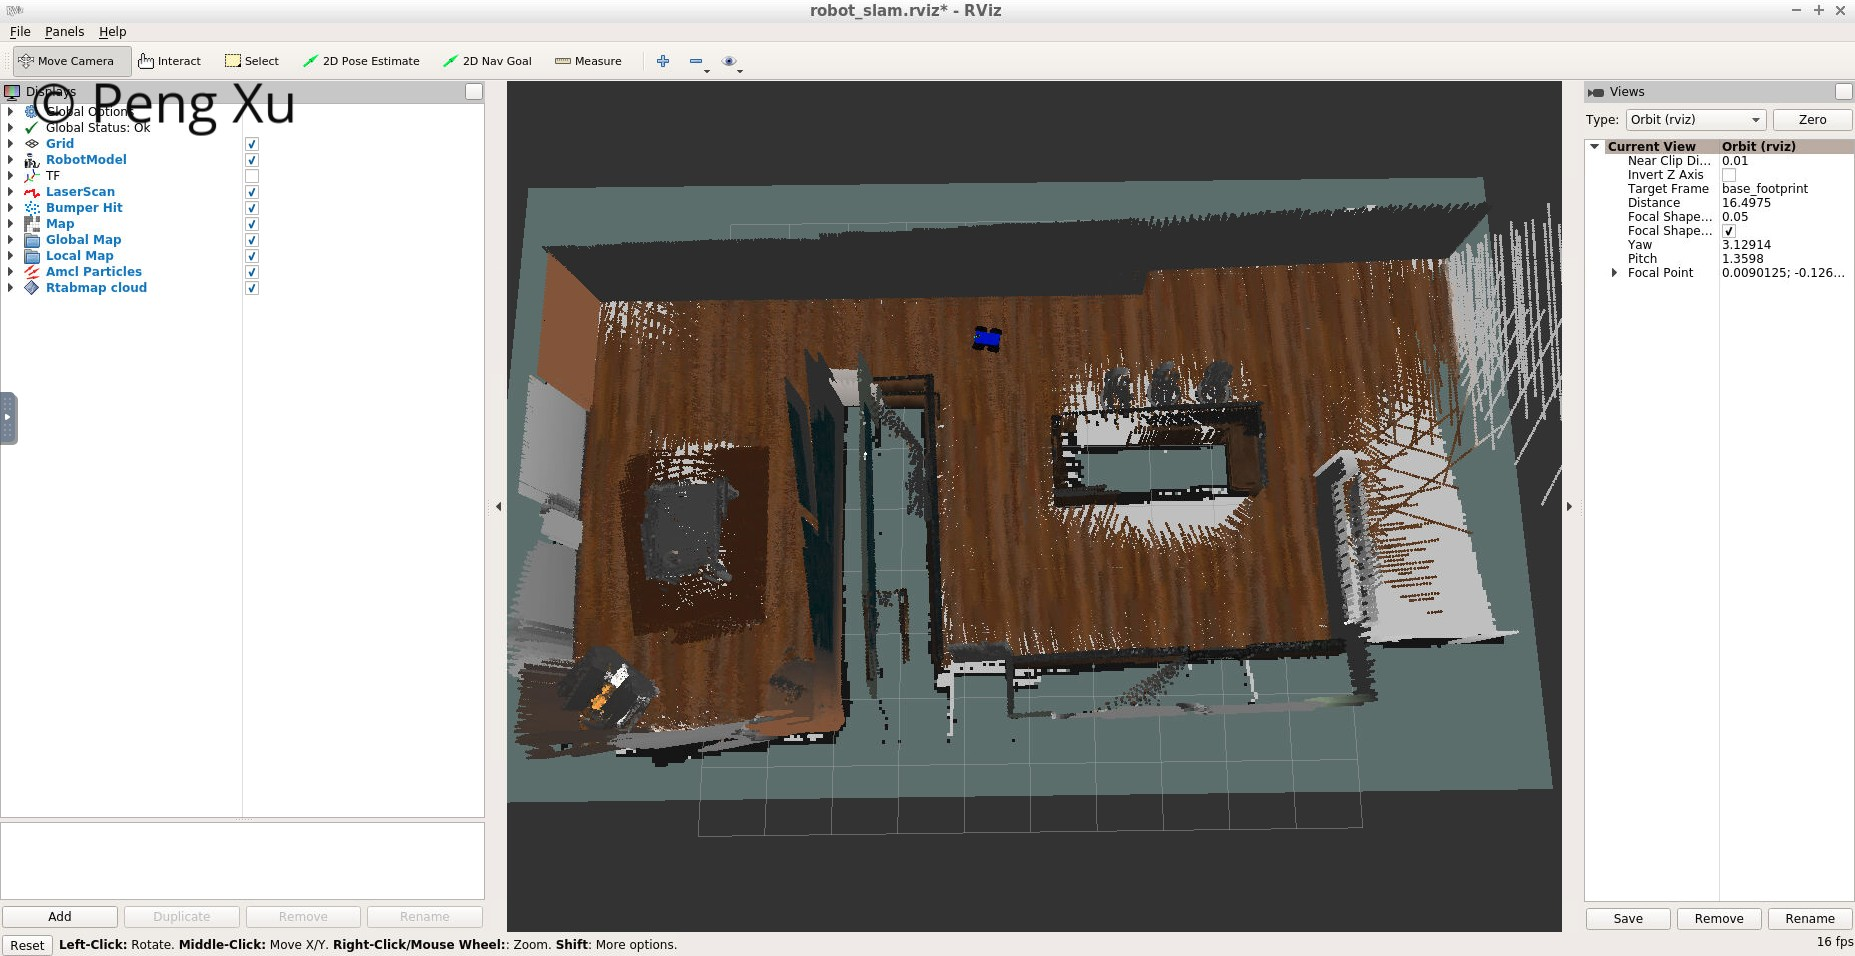
\includegraphics[width=\linewidth]{images/kitchen-rviz.png}
      \caption{Rviz Map of Kitchen World}
      \label{fig:kitchen-rviz}
\end{figure}

By inspecting the database created from the experiment run in the kitchen environment, numerous detected loop closures are found. Since the robot revisited the aisle between the counter top and the sink several times, the loop closures correctly identify when the poses around there are similar.

\begin{figure}[thpb]
      \centering
      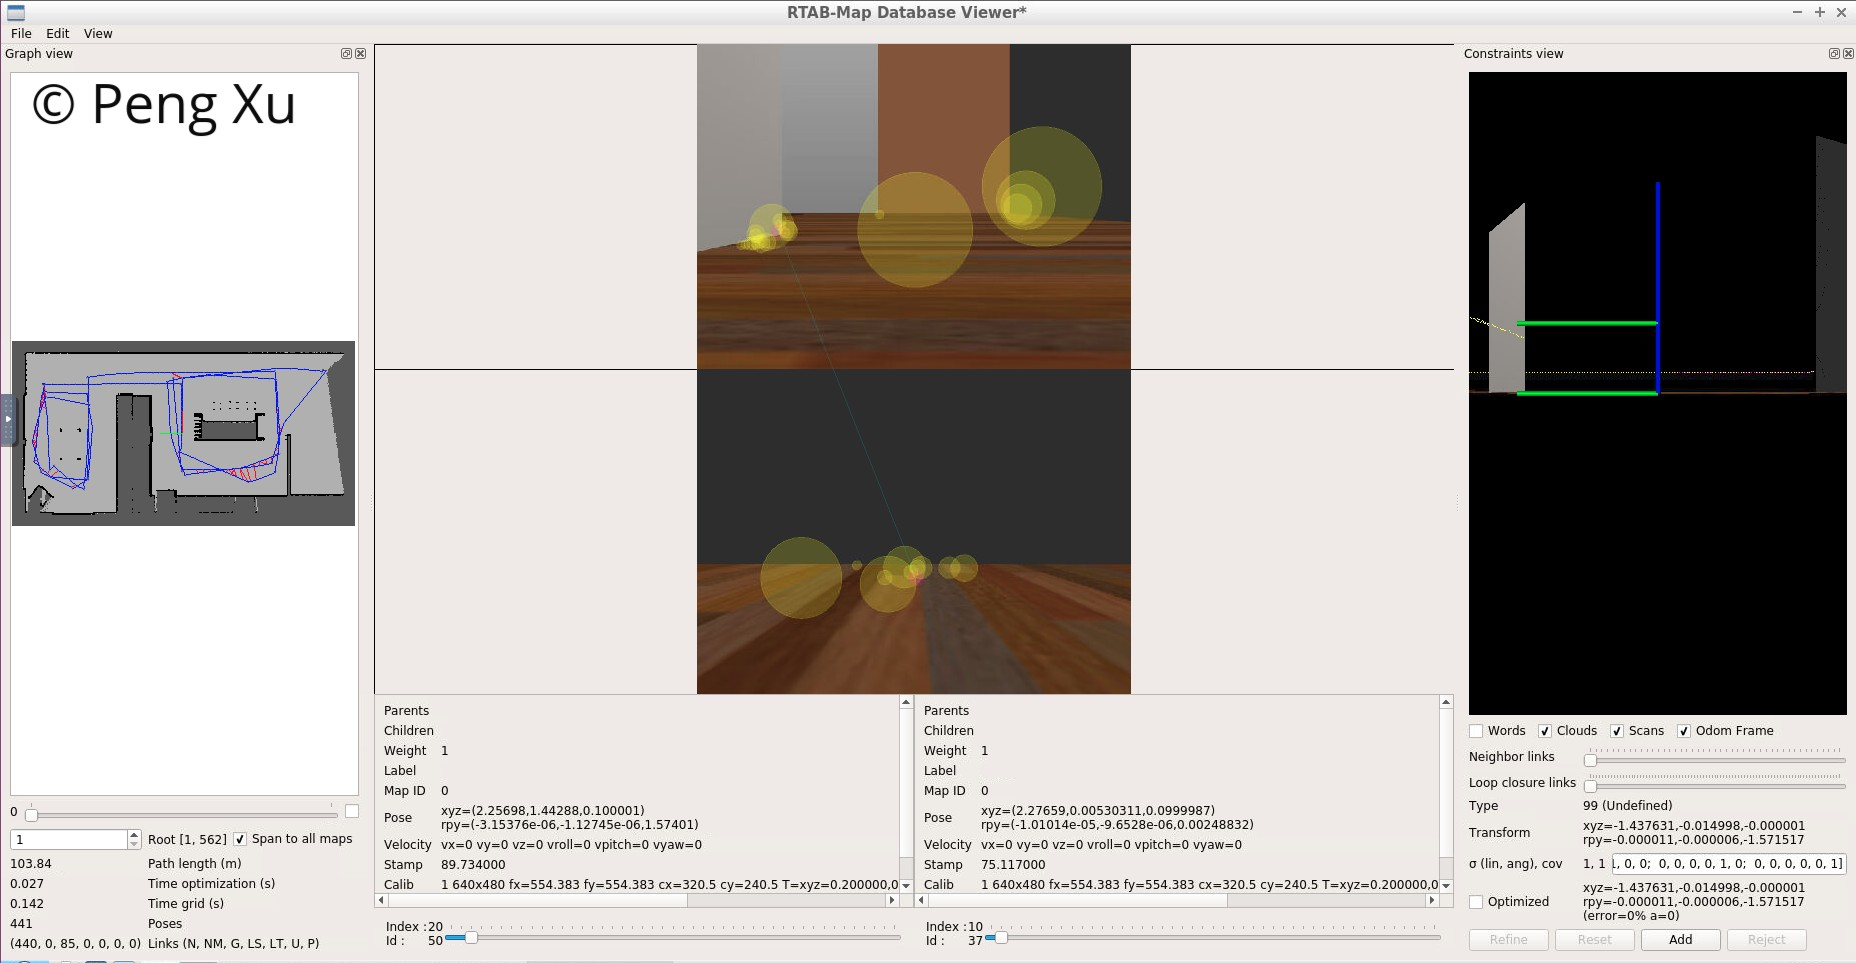
\includegraphics[width=\linewidth]{images/kitchen-database-viewer.png}
      \caption{RTAB Database Viewer 1}
      \label{fig:kitchen-database-viewer}
\end{figure}

\begin{figure}[thpb]
      \centering
      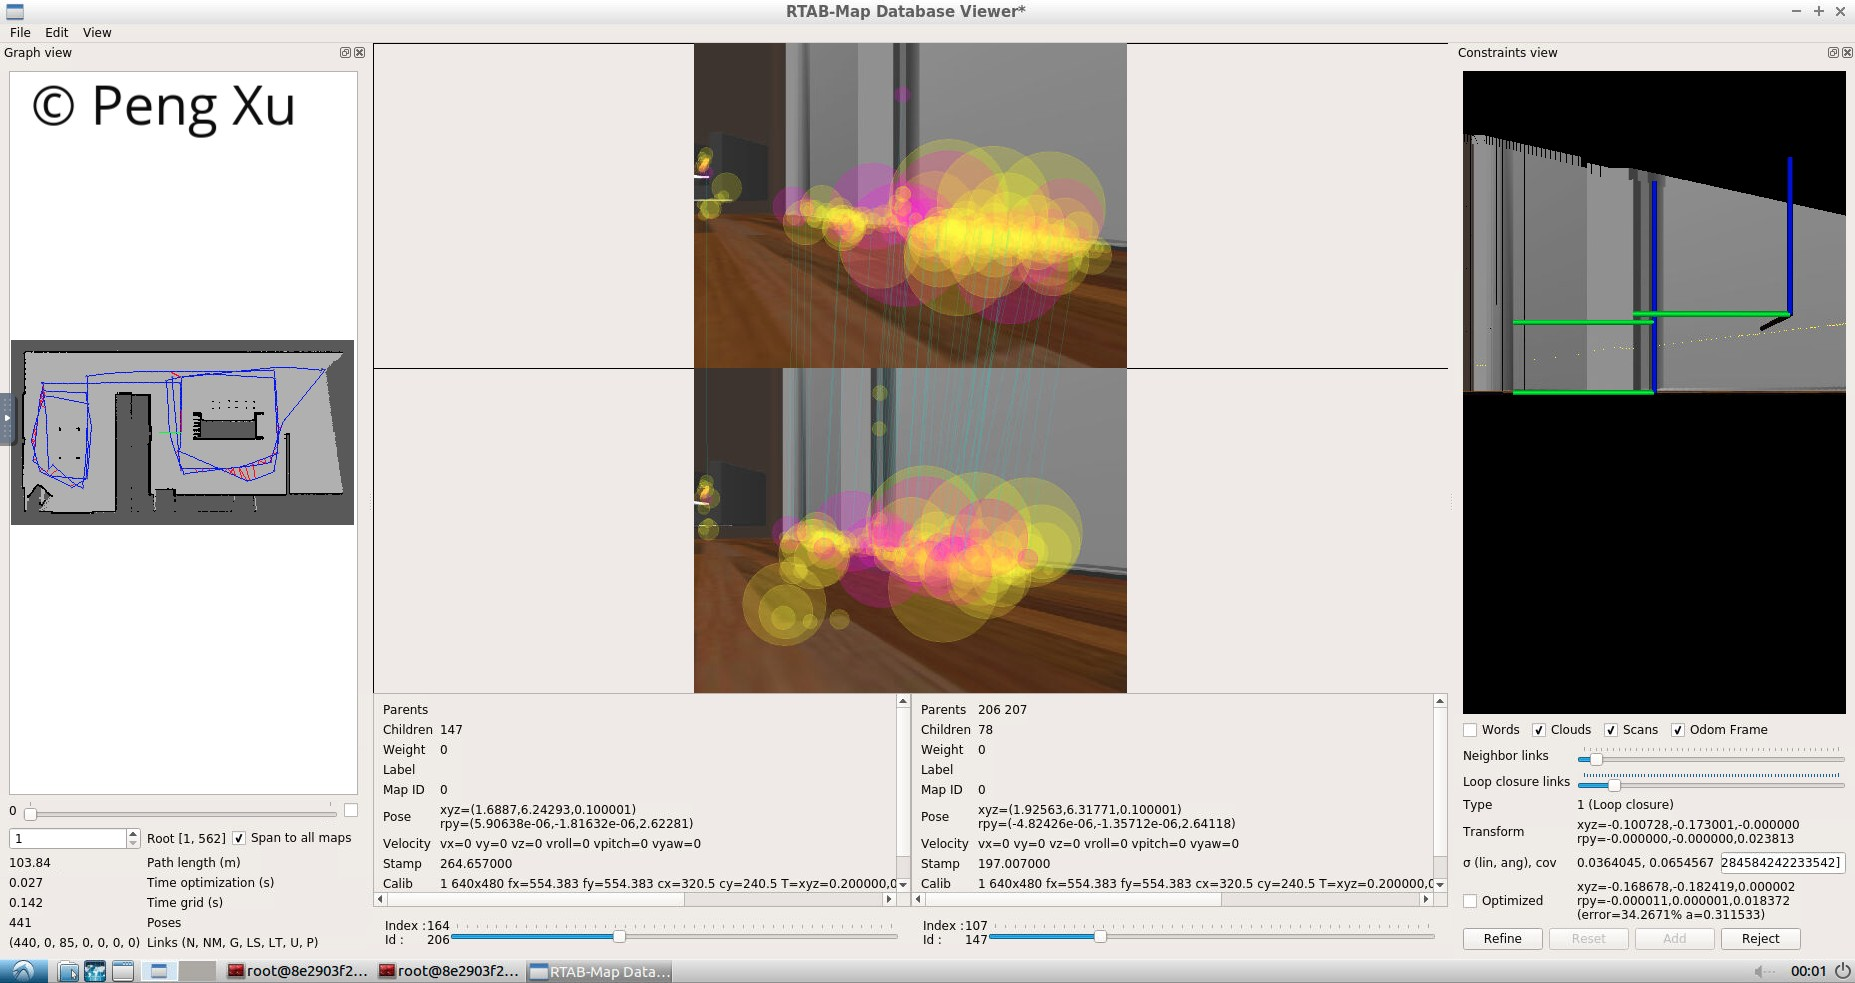
\includegraphics[width=\linewidth]{images/kitchen-database-viewer2.png}
      \caption{RTAB Database Viewer 2}
      \label{fig:kitchen-database-viewer2}
\end{figure}

\subsection{Cafe World}

A cafe world built as in Fig. \ref{fig:cafe-gazebo} was explored by the robot then. The generated 2D map is shown as in Fig. \ref{fig:cafe-rviz}.

\begin{figure}[thpb]
      \centering
      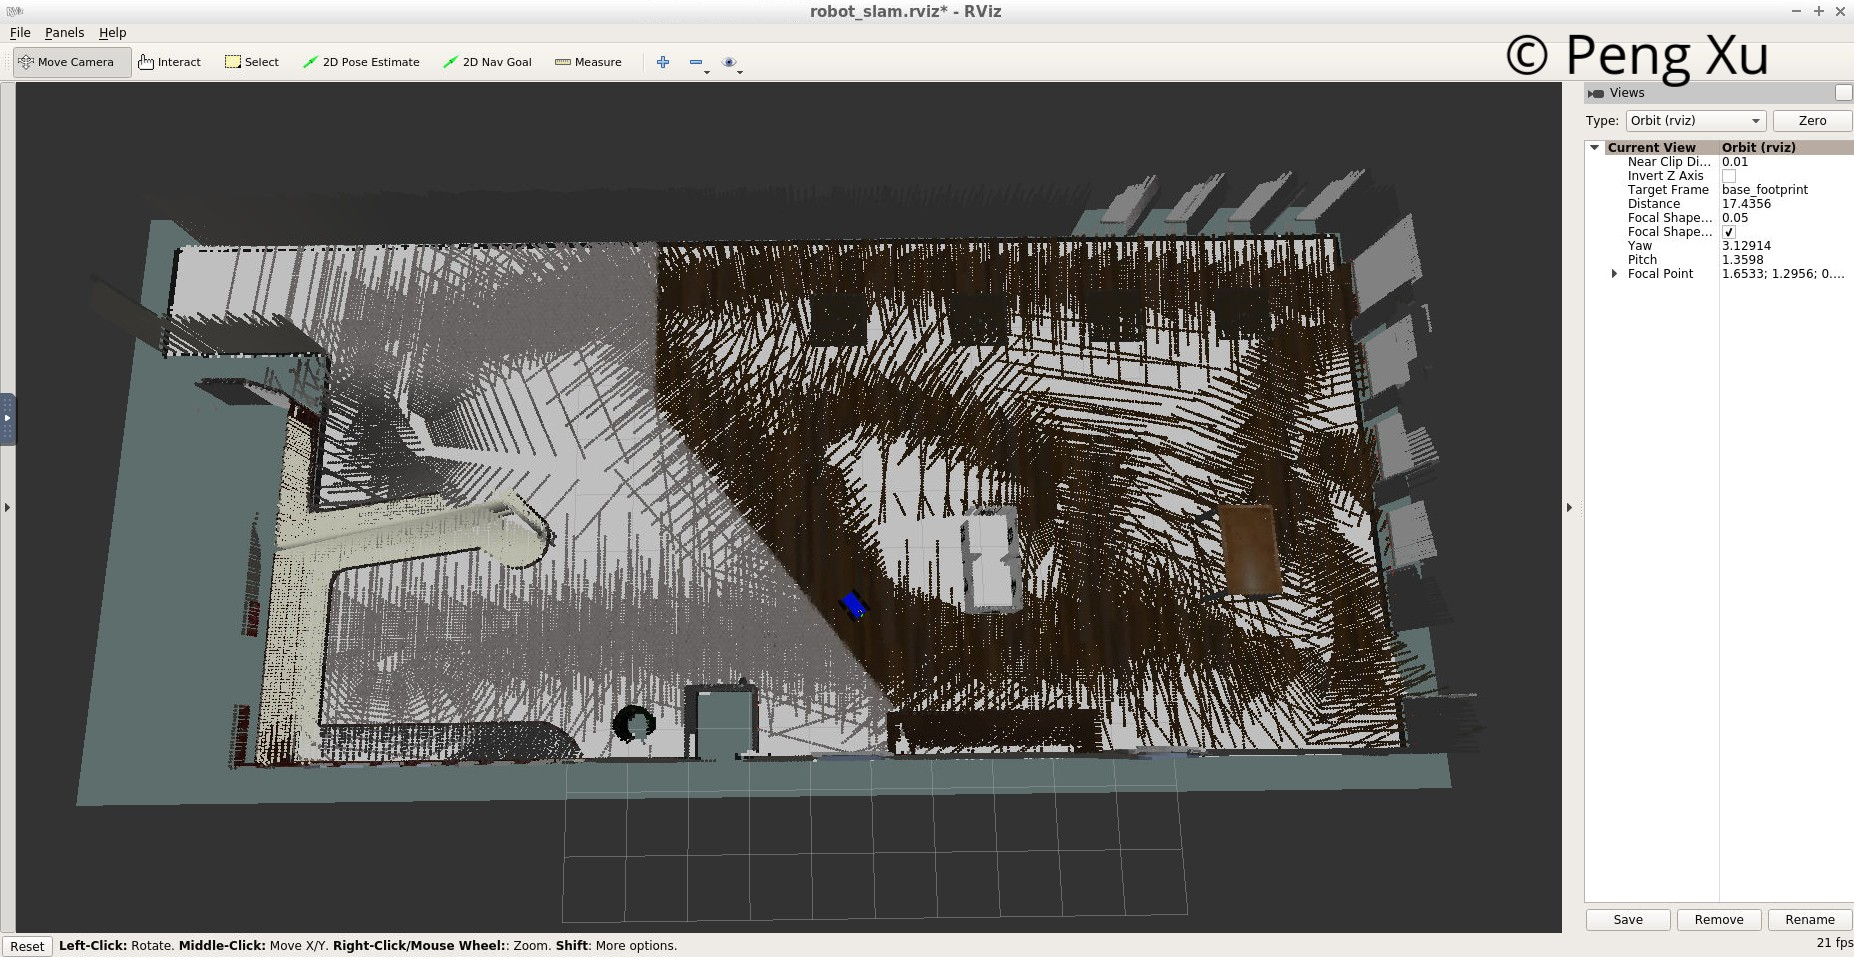
\includegraphics[width=\linewidth]{images/cafe-rviz.png}
      \caption{Rviz Map of Cafe World}
      \label{fig:cafe-rviz}
\end{figure}

The example display of RTAB-Map of the cafe world during the exploration is as shown in Fig. \ref{fig:cafe-rtab-map}.

\begin{figure}[thpb]
      \centering
      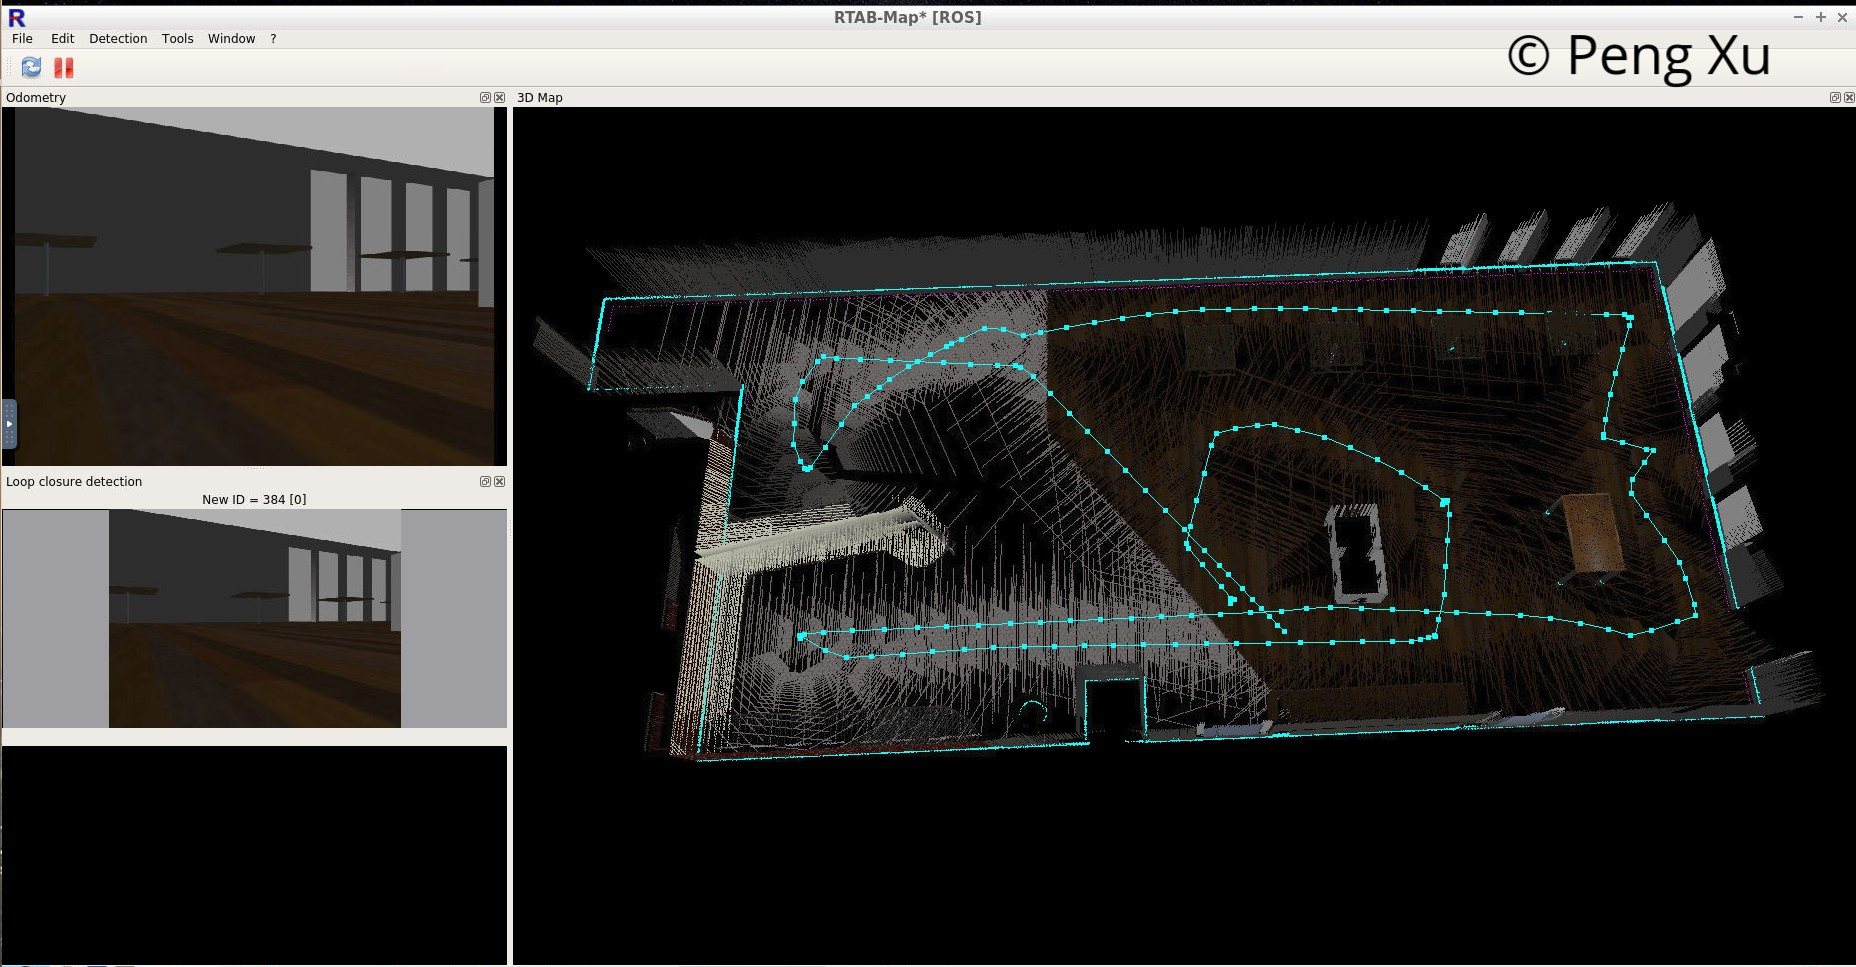
\includegraphics[width=\linewidth]{images/cafe-rtab-map.png}
      \caption{RTAB Map of Cafe World}
      \label{fig:cafe-rtab-map}
\end{figure}

\section{Discussion}

Mapping the provided kitchen environment was an easier task than mapping the customized environment. The robot was able to perform the mapping task accurately enough around the room, while it took me several rounds of trial and error to make the mapping result usable in the cafe world environment. The kitchen world environment is conducive to the success of the RTAB map because it contains feature-rich objects such as chairs and sofa. In addition, even though the wood tiles are repetitive and the walls are feature-less, the surrounding objects are dense enough for the robot to consistently map the environment even when looking towards corners of the rooms.

The robot failed a few times in the cafe world environment since the RTAB map algorithm produced false positives of loop closures. For example, when the camera is facing the stone wall, it detects a lot of small features on the wall. However, when the camera is facing another section of the stone wall, the algorithm would identify them as the same section, and the 3D map would be repeated while rotated to product unusable maps such as the one demonstrated in the lesson. 

\section{Future work}

RTAB map uses the Bag of Words approach to identify reoccurring objects. However, the method needs tuning and sometimes produce false positives of loop closures. When such false positives occur, the created map would be heavily distorted and unable to be used. Object detection and classification algorithms with better precision, such as deep neural network, might be able to reduce false positives and enable the robot to map similarly well in less feature-rich environments.

In addition, the RTAB map does not perform well when there are dynamic objects in the environment. Since the RTAB map assumes the objects to be static in the environment, when it detects an object appearing at different locations, it will be unable to produce the correct constraints and result in a low quality map. A more advanced detection algorithm would be required to distinguish a moving object from a dynamic object.

In the future, along with further effort in simulation environment, a strong interest is to make it work on a real mobile robot. Visual SLAM would be continuously being an essential technique to make the robot more and more friendly.

\end{document}